% Copyright 2004 by Till Tantau <tantau@users.sourceforge.net>.
%
% In principle, this file can be redistributed and/or modified under
% the terms of the GNU Public License, version 2.
%
% However, this file is supposed to be a template to be modified
% for your own needs. For this reason, if you use this file as a
% template and not specifically distribute it as part of a another
% package/program, I grant the extra permission to freely copy and
% modify this file as you see fit and even to delete this copyright
% notice. 

\documentclass{beamer}
\usepackage{graphicx}
\usepackage{epstopdf}
\usepackage{xcolor}
\usepackage{textcomp}
\usepackage{listings}
\graphicspath{ {resources/} }

\newenvironment{figure*}%
{\begin{figure}}
{\end{figure}}

% Required for the Table
\usepackage{csvsimple}
\usepackage{booktabs}
\usepackage{multirow}
\usepackage{hhline}

\definecolor{darkgreen}{RGB}{0,96,32}

% There are many different themes available for Beamer. A comprehensive
% list with examples is given here:
% http://deic.uab.es/~iblanes/beamer_gallery/index_by_theme.html
% You can uncomment the themes below if you would like to use a different
% one:
%\usetheme{AnnArbor}
%\usetheme{Antibes}
%\usetheme{Bergen}
%\usetheme{Berkeley}
%\usetheme{Berlin}
%\usetheme{Boadilla}
%\usetheme{boxes}
%\usetheme{CambridgeUS}
%\usetheme{Copenhagen}
%\usetheme{Darmstadt}
%\usetheme{default}
%\usetheme{Frankfurt}
%\usetheme{Goettingen}
%\usetheme{Hannover}
%\usetheme{Ilmenau}
%\usetheme{JuanLesPins}
%\usetheme{Luebeck}
\usetheme{Madrid}
%\usetheme{Malmoe}
%\usetheme{Marburg}
%\usetheme{Montpellier}
%\usetheme{PaloAlto}
%\usetheme{Pittsburgh}
%\usetheme{Rochester}
%\usetheme{Singapore}
%\usetheme{Szeged}
%\usetheme{Warsaw}

\lstdefinestyle{customc}{
  belowcaptionskip=1\baselineskip,
  breaklines=true,
  frame=L,
  xleftmargin=\parindent,
  language=C,
  showstringspaces=false,
  basicstyle=\footnotesize\ttfamily,
  keywordstyle=\bfseries\color{green!40!black},
  commentstyle=\itshape\color{purple!40!black},
  identifierstyle=\color{blue},
  stringstyle=\color{orange},
  morekeywords={},
  moredelim=[is][\color{red}]{|}{|}
}

\lstdefinestyle{customasm}{
  belowcaptionskip=1\baselineskip,
  frame=L,
  xleftmargin=\parindent,
  language=[x86masm]Assembler,
  basicstyle=\footnotesize\ttfamily,
  commentstyle=\itshape\color{purple!40!black},
}

\lstset{escapechar=@,style=customc,moredelim=[is][\color{red}]{|}{|}}

\setbeamertemplate{caption}[numbered]

\title{Efficiently Detecting Use-after-Free Exploits \ \ \\in Multi-threaded Programs}

% A subtitle is optional and this may be deleted
\subtitle{Master Project Presentation}

\author{Vinod ~Nigade} 
% - Give the names in the same order as the appear in the paper.
% - Use the \inst{?} command only if the authors have different
%   affiliation.

\institute[VU, Amsterdam] % (optional, but mostly needed)
{
  %
  Supervised and Guided by: \\
  \texttt{Erik van der Kouwe}, \texttt{Cristiano Giuffrida}  \\
  Vrije University, Amsterdam
}
% - Use the \inst command only if there are several affiliations.
% - Keep it simple, no one is interested in your street address.

\date{14\textsuperscript{th} September, 2016}
% - Either use conference name or its abbreviation.
% - Not really informative to the audience, more for people (including
%   yourself) who are reading the slides online

\subject{System Security}
% This is only inserted into the PDF information catalog. Can be left
% out. 

% If you have a file called "university-logo-filename.xxx", where xxx
% is a graphic format that can be processed by latex or pdflatex,
% resp., then you can add a logo as follows:

\pgfdeclareimage[height=0.5cm]{VU-Logo-pdf}{VU-Logo-pdf.pdf}
\logo{\pgfuseimage{VU-Logo-pdf}}

% Delete this, if you do not want the table of contents to pop up at
% the beginning of each subsection:
%\AtBeginSubsection[]
%{
  %\begin{frame}<beamer>{Outline}
    %\tableofcontents[currentsection,currentsubsection]
  %\end{frame}
%}

% Let's get started
\begin{document}

\begin{frame}
  \titlepage
\end{frame}

\begin{frame}{Outline}
  \tableofcontents
  % You might wish to add the option [pausesections]
\end{frame}

% Section and subsections will appear in the presentation overview
% and table of contents.
\section{Introduction}

%\subsection{Dangling Pointer}

\begin{frame}{Use-after-Free}{Background}
\begin{block}{Dangling Pointer}
Pointer that points to freed memory
\end{block}
\begin{block}{Use-after-Free}
\begin{itemize}
\item Referencing memory after it has been freed
\item Leads to program crash, data corruption, arbitrary code execution
\item Highly critical and popular attack vector
\item Common coding practice: Set pointer to benign value NULL when object is freed
\end{itemize}
\end{block}
\end{frame}

\begin{frame}{Use-after-Free}{Mitigation Techniques}
\begin{itemize}
\item Static Analysis \\
\begin{itemize}
\item Source code or Binary analysis 
\item Hard to find: Needs complex inter-procedural and points-to analysis  \\
\end{itemize}
\item Dynamic Analysis \\
\begin{itemize}
\item Track run-time pointer-object relationship
\item Introduces huge run-time overhead or limited applicability
\item DangNull \cite{lee2015dangnull} has on an average of {\color{red}$80\%$} run-time overhead, FreeSentry \cite{younan2015freesentry} has $25\%$ but with {\color{red}no thread-safety}.
\end{itemize}
\end{itemize}

\end{frame}

%\subsection{Use-after-Free impact}

% You can reveal the parts of a slide one at a time
% with the \pause command:

%\subsection{Mitigation Techniques}

\section{Background}

\begin{frame}{Background}{Insert Tracking Functions}
\lstinputlisting[title=Static Instrumentation, language=C]{Source/static_reg.c}
\end{frame}

\begin{frame}{Background}{Run-time Tracking}
\begin{minipage}{0.45\textwidth}
\texttt{\color{red}track\_ptr(ptr,obj)}
\begin{itemize}
\item Find metadata given any inbound object address \\(e.g. \texttt{\color{blue}p}, \texttt{{\color{blue}p} + 10})
\item Remove \texttt{ptr} from old object metadata /* Optional */
\item Store \texttt{ptr} info in metadata
\end{itemize}
\begin{figure}[h]
	\centering
	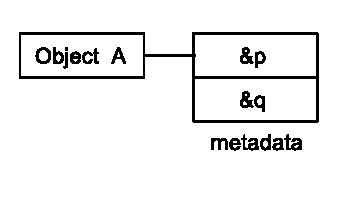
\includegraphics[scale=0.7]{pointer_tracking.eps} 
\end{figure}
\end{minipage}%
\hfill
\begin{minipage}{0.45\textwidth}
\begin{tabular}{|p{\textwidth}}
\texttt{\color{red}nullify\_ptr(obj)}
\begin{itemize}
\item Find metadata given object address
\item Nullify pointers
%\lstinputlisting[style=customc]{Source/ptr_track.c}
\end{itemize}
%\lstinputlisting[style=customc]{Source/ptr_track.c}
\begin{center}
$\texttt{\color{blue}p}\ = \texttt{\textcolor{darkgreen}{NULL}};$ \\
$\texttt{\color{blue}q}\ = \texttt{\textcolor{darkgreen}{NULL}};$
\end{center}
\end{tabular}
\end{minipage}%

\end{frame}

\begin{frame}{Background}{MetAlloc}
\begin{itemize}
\item Trees, Hashtables etc. used to store and retrieve pointer-object relationship
\item Requirement: fast metadata lookups (support range queries) and allocations with low memory overhead
\item MetAlloc \cite{istvan2016metalloc} shadow memory technique with fixed metadata lookup time.
\item Supports range queries, variable and fixed compression ratio, uniform metadata tracking 
\end{itemize}
\end{frame}

\begin{frame}{Background}{FreeSentry scheme using MetAlloc}
\begin{figure}[h]
	\centering
	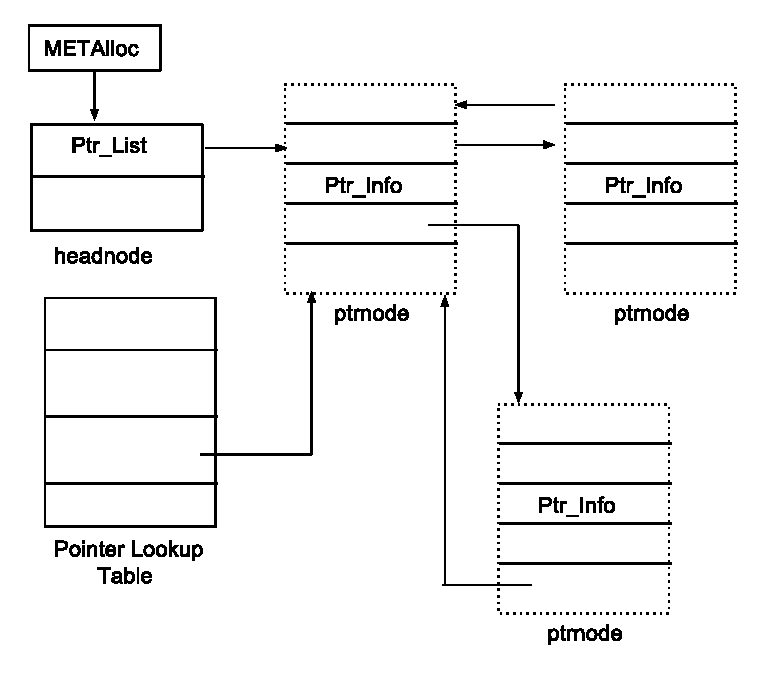
\includegraphics[scale=0.5]{metalloc-freesentry.eps} 
	\caption{Data Structure design} 
\end{figure}

\end{frame}

\section{Problem Statement}
\begin{frame}{Problem Statement}
	\begin{itemize}
	\item State-of-the-art complete systems incur huge run-time overhead. 
	\item Not all pointers (e.g. Stack and Global) are supported 
	\item Large and complex applications like Web-Servers, Browsers can be multi-threaded
	\end{itemize}			
		
	\begin{block}{Problem}
		No efficient system to prevent Use-after-Free exploits in multi-threaded programs 
	\end{block}
\end{frame}

\section{Our Approach}
\begin{frame}{Our Approach}{Overview}
\begin{block}{In a simple Design}
Need list of pointers per object.
\end{block}
\begin{itemize}
\item Large number of pointer tracking calls 
\item No need to remove pointer from old object list i.e. Pointer-to-object metadata not needed.
\item metadata lookups: $1)$ Object-to-metadata
\end{itemize}
\end{frame}

\begin{frame}{Our Approach}{Data Structures}
\begin{figure}[h]
	\centering
	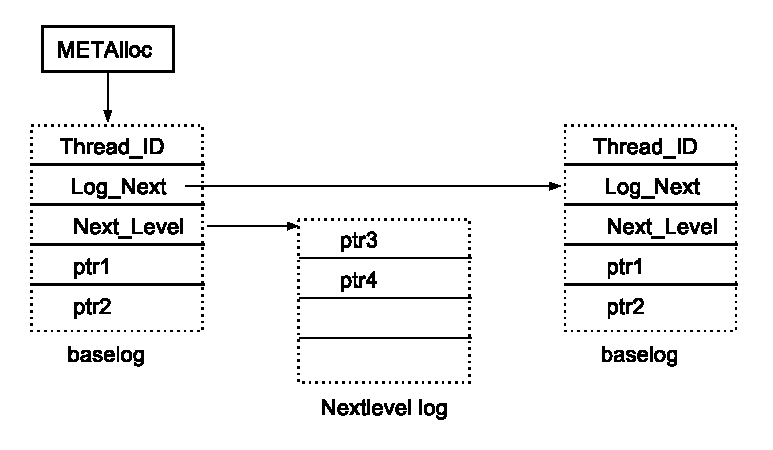
\includegraphics[width=3.5in]{dangsang_design.eps} 
	\caption{per-Object data structure}
\end{figure}
\end{frame}

\begin{frame}{Our Approach}

\begin{block}{Log overflow}
\begin{itemize}
\item Second level indirect log 
\item Exponential log resize
\end{itemize}
\end{block}

\begin{block}{\emph{N}-Lookbehind}
\begin{itemize}
\item Lookbehind last \emph{N} entries in the log
\item Avoid duplicate pointer logging
\end{itemize}
\end{block}

\begin{block}{Garbage Collection}
\begin{itemize}
\item Treat log as a circular buffer
\item Remove old stale pointers
\end{itemize}
\end{block}
\end{frame}

\begin{frame}{Our Approach}{Application Compatibility}
	
\begin{block}{Pointers subtraction}
\begin{itemize}
\lstinputlisting[style=customc]{Source/ptr_sub.c} 
	
\item Set uppermost bit to $1$ i.e. $p\ =\ p\ |\ 0x8000000000000000$
\end{itemize}
\end{block}

\begin{block}{Off-by-one byte}
\begin{itemize}
\item STL Vector\{\texttt{start}, \texttt{next}, \texttt{end}\}, \texttt{next} and \texttt{end} may point out-of-bound by one byte
\item Increase object allocation size by one.
\end{itemize}
\end{block}
\end{frame}

%\begin{frame}{Our Approach}{Application Compatibility}
%\begin{block}{GCC}
%\lstinputlisting[style=customc]{Source/gcc_alloc.c}
%\lstinputlisting[style=customc]{Source/gcc_free.c}
%\end{block}
%\end{frame}

\section{Evaluation}
\begin{frame}{Evaluation}{Thread-Safety}
\begin{block}{}
Average run-time overhead: With thread-safety ({\color{red}$69.6\%$}) and without ({\textcolor{darkgreen}{$33.2\%$}})
\end{block}

\begin{figure}[h]
	\centering
	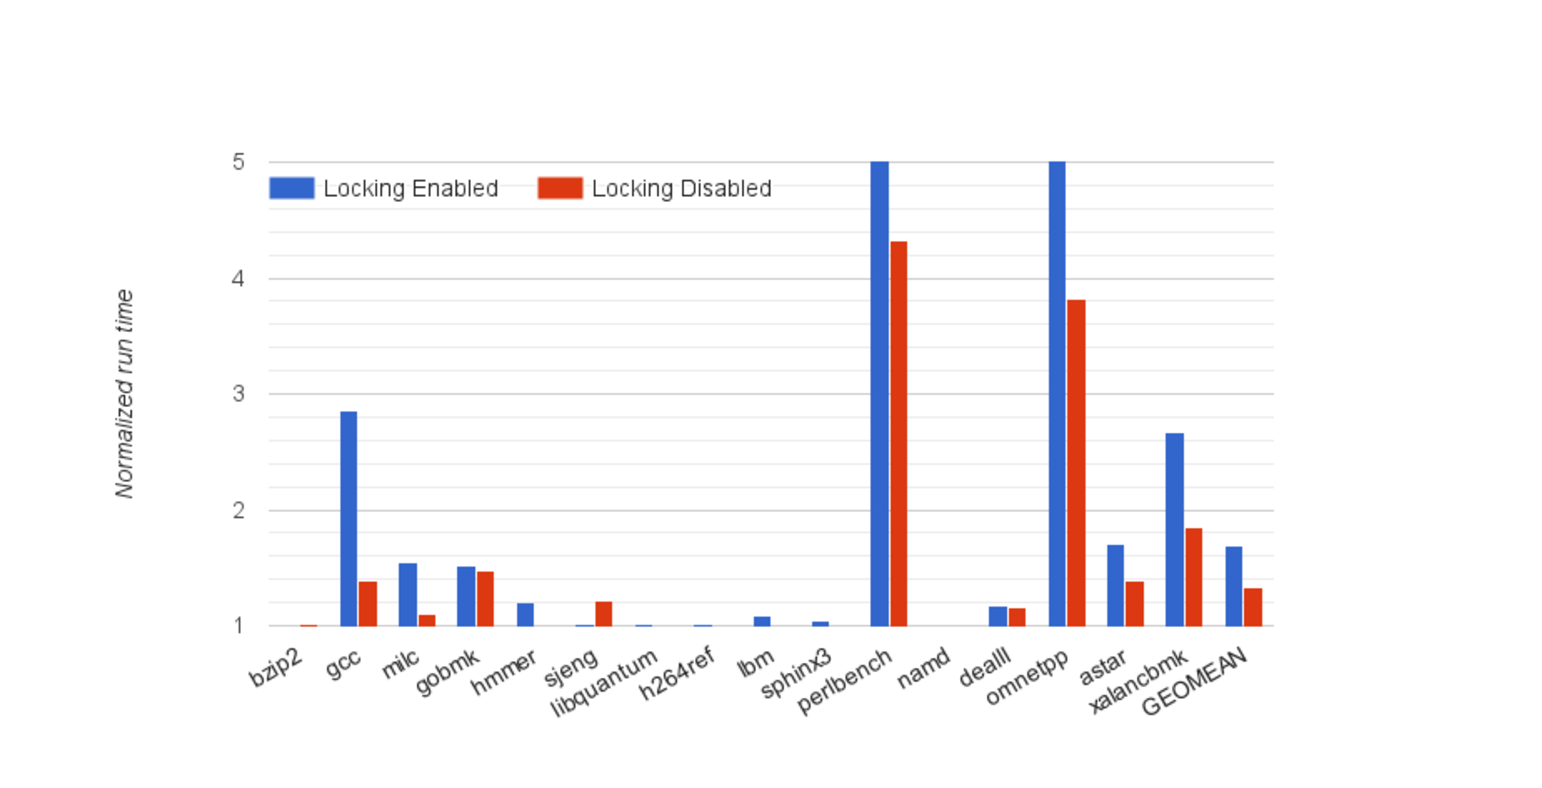
\includegraphics[width=4.5in]{metalloc-freesentry_graph.eps} 
	%\caption{FreeSeentry scheme using MetAlloc}
\end{figure}

\end{frame}

\begin{frame}{Evaluation}{Performance Analysis}
\begin{block}{}
\begin{itemize}
\item All benchmarks, $43.9\%$ (only heap pointers), $47.6\%$ (all pointers)
\item Without perlbench ;), $34.3\%$ (only heap pointers), $37.2\%$ (all pointers)
\end{itemize}  
\end{block}

\begin{figure}[h]
	\centering
	\includegraphics[width=4.5in]{plots/spec_graph.png} 
\end{figure}
\end{frame}

\begin{frame}{Evaluation}{Performance Analysis}
\begin{block}{}
On an average, Web Servers have 12.8\% throughput degradation and negligible service latency
\end{block}
\begin{figure}[h]
	\centering
	\includegraphics[width=2.5in]{Tables/server_perf.eps} 
\end{figure}
\end{frame}

\begin{frame}{Evaluation}{Correctness}
\begin{block}{}
CVE 2010­2939: OpenSSL\_1.0.0a 'ssl3\_get\_key\_exchange()' Use-­after­Free memory 
corruption vulnerability
\end{block}
\begin{table}
\begin{tabular}{l|r}
\textbf{Without protection} & \textbf{With protection} \\
\bottomrule
\footnotesize {
\begin{tabular}{@{}l@{}}
46912496417824:error:0407006A:rsa\\ routines:\\RSA\_padding\_check\_PKCS1\_type\_1:block \\type 
is not 01:rsa\_pk1.c:100: \\
46912496417824:error:04067072:rsa \\routines:RSA\_EAY\_PUBLIC\_DECRYPT:\\padding check 
failed:rsa\_eay.c:699: \\
46912496417824:error:1408D07B:SSL \\routines:SSL3\_GET\_KEY\_EXCHANGE:bad\\ 
signature:s3\_clnt.c:1570: 
\end{tabular} } & 
\footnotesize {
\begin{tabular}{@{}l@{}} 
src/tcmalloc.cc:290] Attempt to \\free invalid pointer \\ {\color{green}0x80000000022ba510} \\
./runclient: line 9: 20200 Aborted  \\               \$OPENSSL s\_client ­connect  \\
localhost:\$SERVER\_PORT \end{tabular} }

\end{tabular}
\end{table}
\end{frame}

\section{Limitations and Future Work}
\begin{frame}{Limitations and Future Work}
\begin{itemize}
\item No stack objects are supported
\item Sophisticated and advanced static instrumentation (e.g. avoid tracking for simple pointer arithmetic, i.e. p++)
\item Opt-out selective functions from instrumentation. 
\item Implementation specific: Skip MetAlloc lookups to ignore Stack and Global objects 
\end{itemize}
\end{frame}

% Placing a * after \section means it will not show in the
% outline or table of contents.
\section*{Conclusion}

\begin{frame}{Conclusion}
\begin{block}{Practical and Complete}
Our Use-after-Free detection system is practical and complete compared to state-of-the-art.
\begin{itemize}
\item DangNull: $80\%$, FreeSentry: $25\%$
\item Our Approach: $47.6\%$ (all pointers), $43.9\%$ (heap pointers)
\item Without perlbench: $37.2\%$ (all pointers), $34.3\%$ (heap pointers) 
\end{itemize}
\end{block}

 
\end{frame}



% All of the following is optional and typically not needed. 
\appendix
\section<presentation>*{\appendixname}
\subsection<presentation>*{For Further Reading}

%\begin{frame}[allowframebreaks]
%  \frametitle<presentation>{Referred Literature}
       %\bibliographystyle{apalike}
       %\bibliography{refs.bib}
     
	%\tiny{$\dag$  \url{http://www.mit.edu/~mnick/talks/hole-aaai16.pdf}}
%\end{frame}

\begin{frame}{Extra Slides}{Pointer Patterns}
\begin{figure*}[!t]
\center
  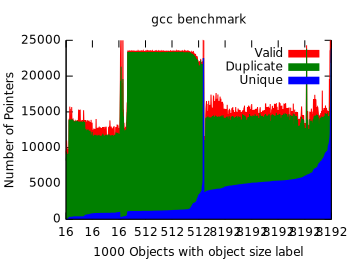
\includegraphics[width=1.6in,height=1.4in,keepaspectratio]{plots/gcc_pointerpattern.pdf}
  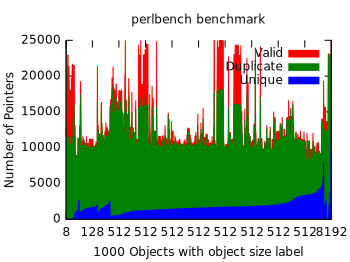
\includegraphics[width=1.6in,height=1.4in,keepaspectratio]{plots/perlbench_pointerpattern.pdf} \\
  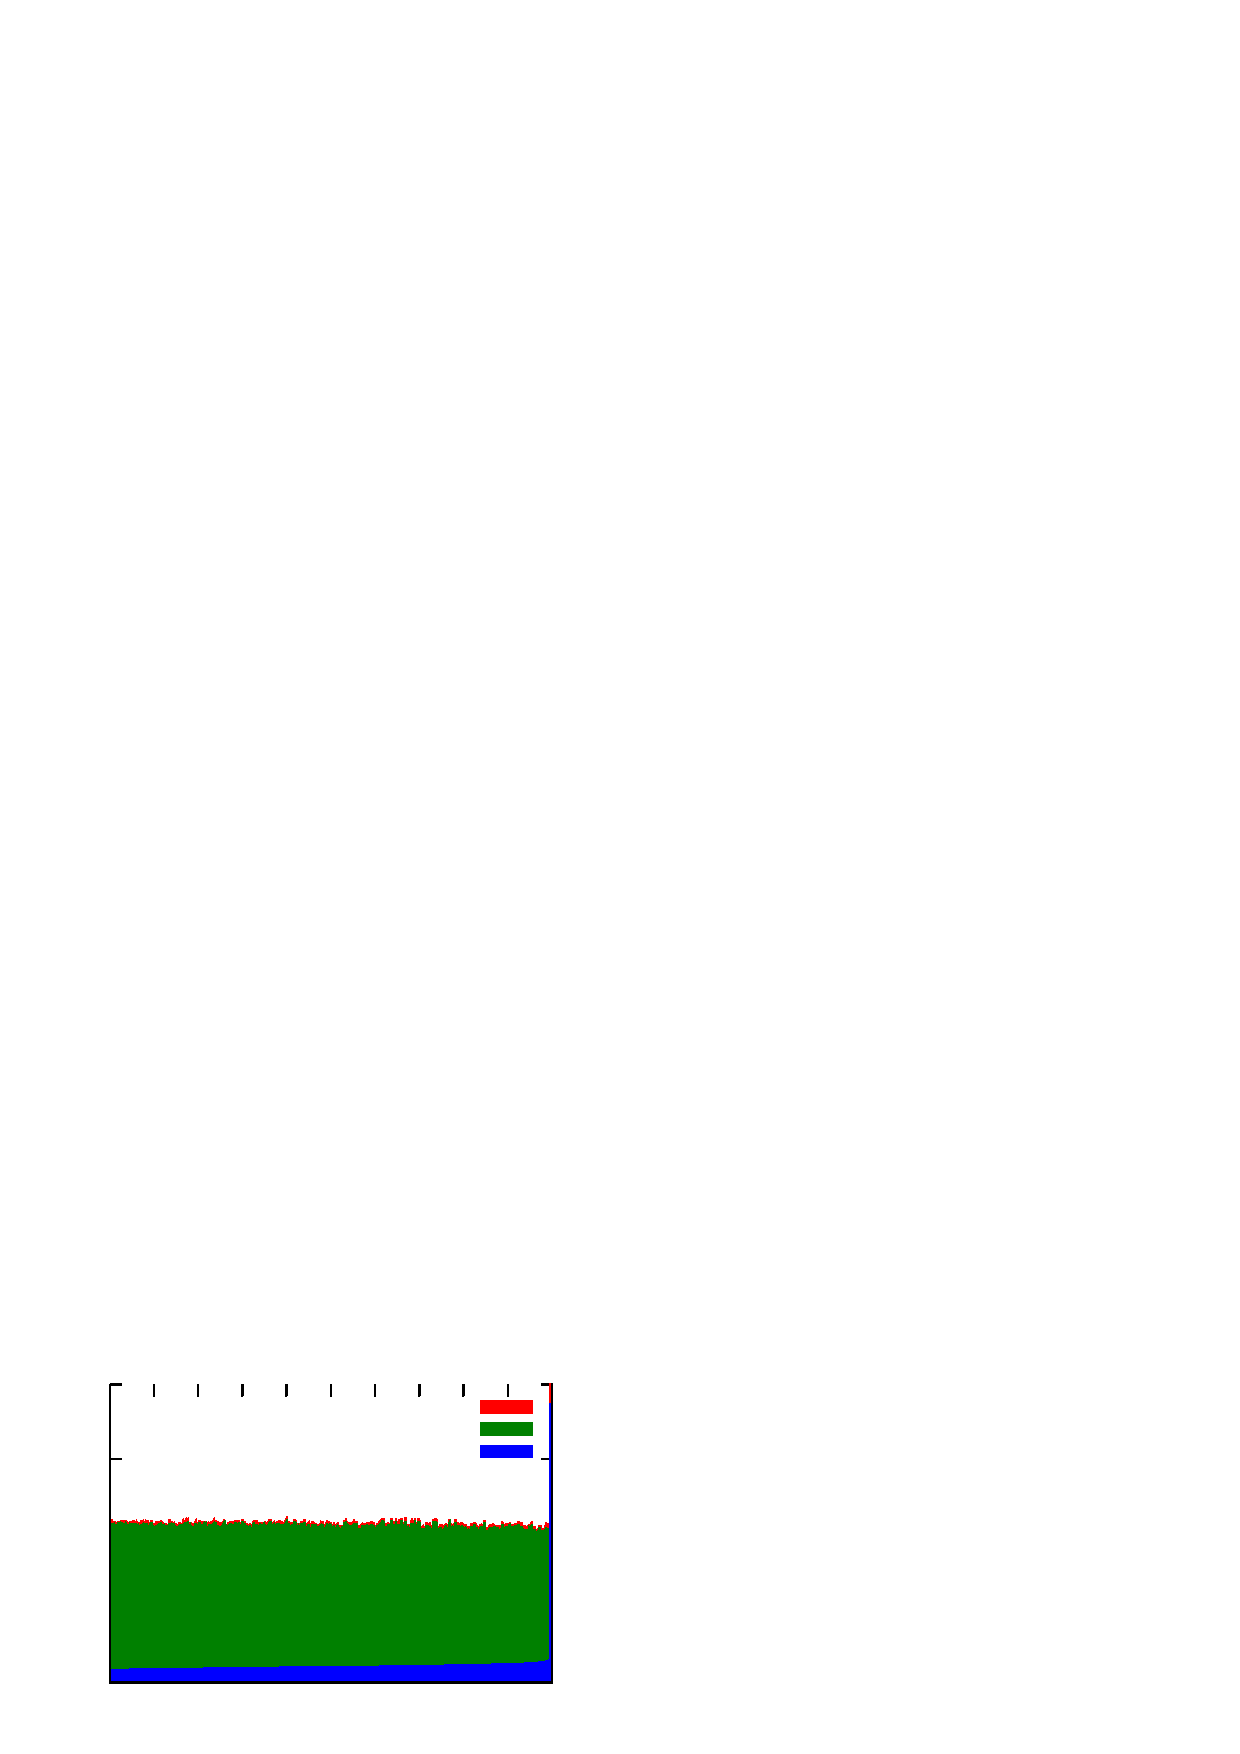
\includegraphics[width=1.6in,height=1.4in,keepaspectratio]{plots/astar_pointerpattern.pdf}
  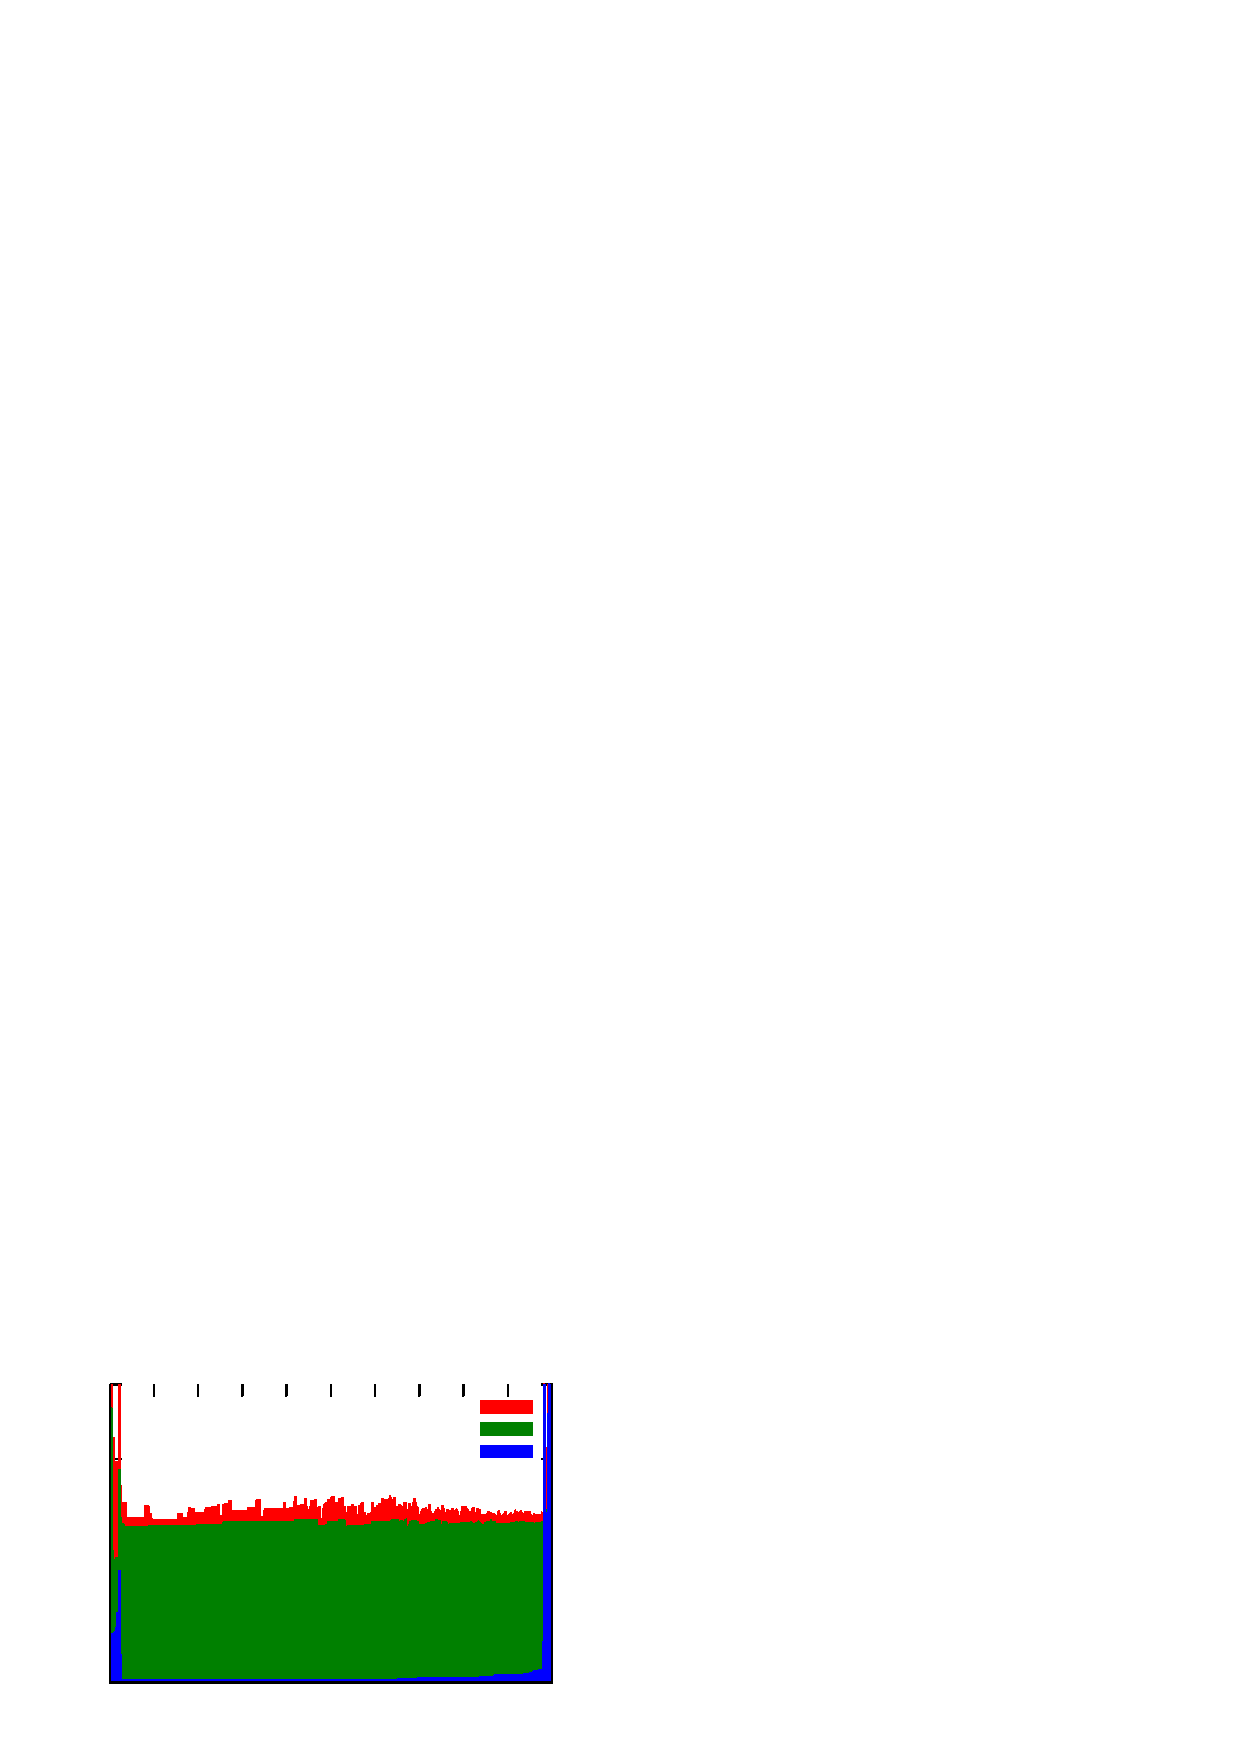
\includegraphics[width=1.6in,height=1.4in,keepaspectratio]{plots/xalancbmk_pointerpattern.pdf}
  
\begin{block}{}
Duplicate and Stale pointers are much higher
\end{block}
  
  %\caption{Pointer registration pattern for the benchmarks that incur huge overhead. First $1000$ baselog overflow numbers are collected. N-Lookbehind value is $4$. Size of the baselog is kept very high to clearly visualize pattern difference.}
  %\label{fig:pointerpattern}
  \vspace{-1em}
\end{figure*}
\end{frame}

\begin{frame}{Extra Slides}{MetAlloc}
\begin{figure}[h]
	\centering
	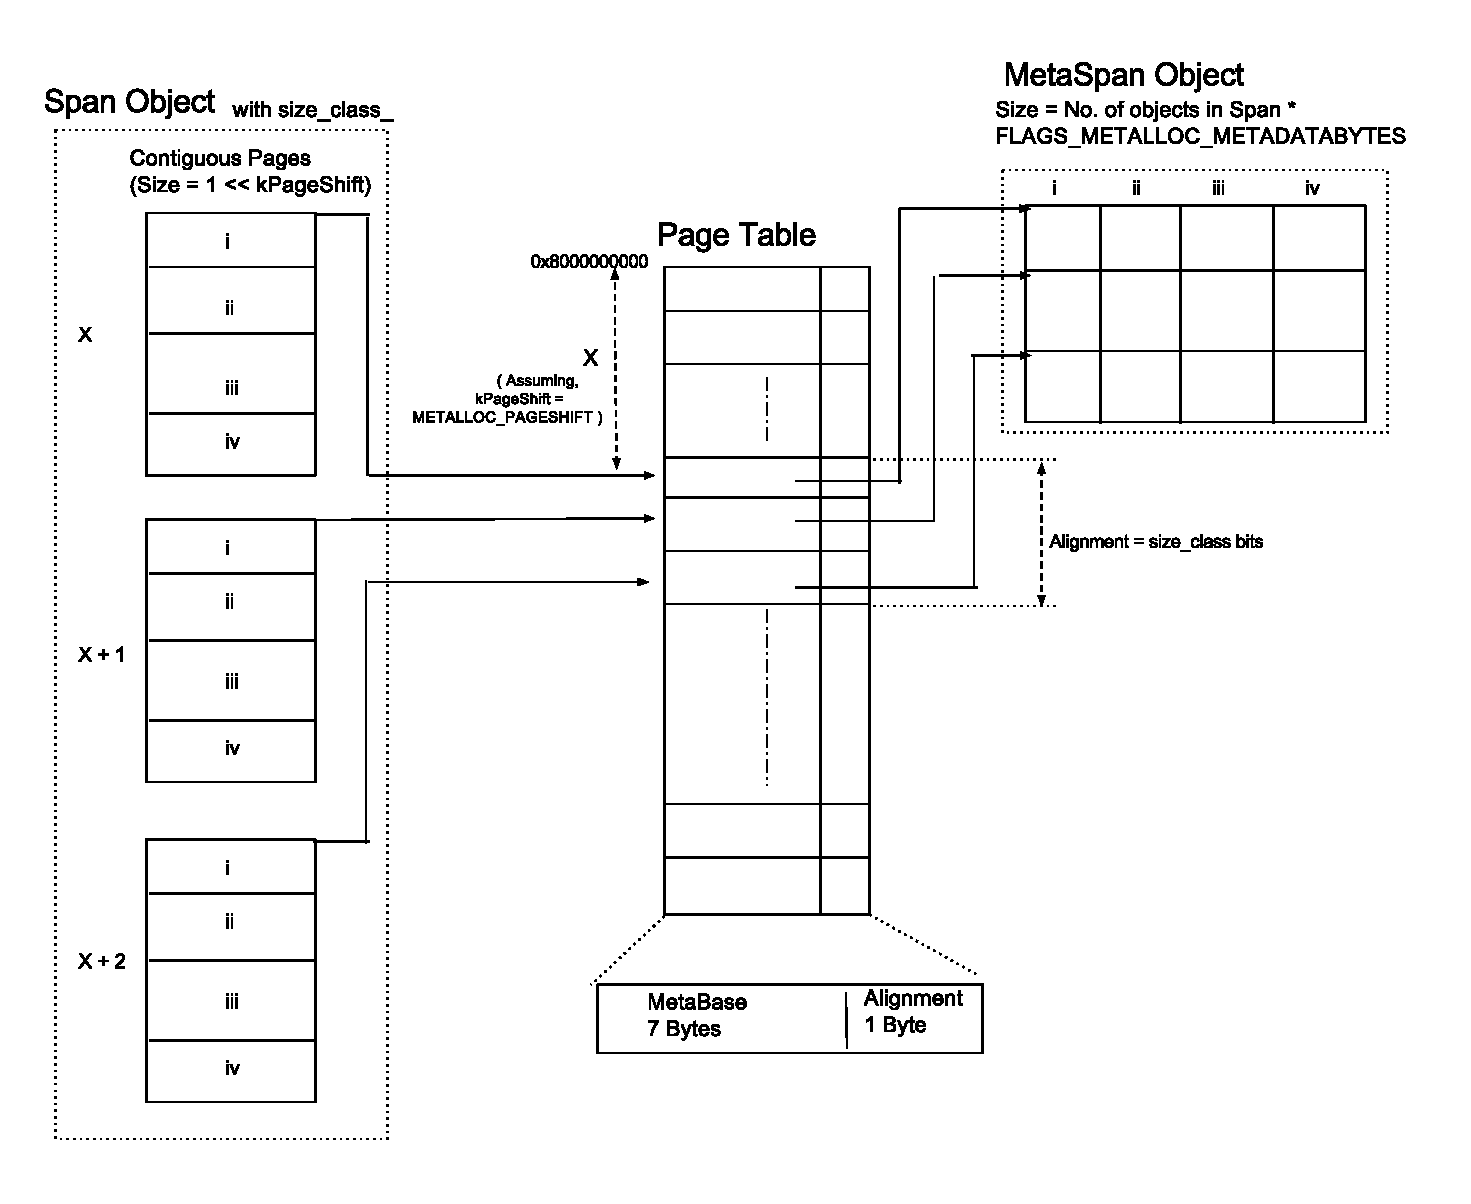
\includegraphics[width=3.5in]{metalloc_heap.eps} 
\end{figure}
\end{frame}

\begin{frame}{Extra Slides}{Stats}
\begin{figure}[h]
	\centering
	\includegraphics[width=5in]{pointer_stats.png} 
\end{figure}
\end{frame}

\bibliographystyle{apalike}
\bibliography{refs.bib}
\end{document}


